\documentclass[a4paper]{article}

\usepackage[T1]{fontenc}
\usepackage{titling}
\usepackage[polish]{babel}
\usepackage{multirow}
\selectlanguage{polish}
\usepackage[utf8]{inputenc}
\usepackage{amsmath}
\usepackage{listings}
\usepackage{graphicx}
\usepackage{framed}
\usepackage{fullpage}
\usepackage{adjustbox}
\usepackage{algpseudocode}
\usepackage{amsthm}
\theoremstyle{plain}
\newtheorem*{theorem*}{Twierdzenie Bézouta}


\setlength{\droptitle}{+10em}
\title{\huge
  Obliczenia naukowe \\
  \large Lista 4}
\author{Arkadiusz Ziobrowski \\ 229728}
\date{}

\begin{document}
\maketitle

\pagebreak




\section{Zadanie pierwsze}

\subsection{Opis problemu}
\paragraph{}
Celem zadania była implementacja funkcji obliczającej ilorazy różnicowe, bez użycia tablicy dwuwymiarowej (macierzy).
\subsection{Rozwiązanie}
\paragraph{}
W języku programowania \texttt{Julia} została zaimplementowana funkcja o następującej sygnaturze:
\begin{center}
\texttt{function ilorazyRoznicowe(x::Vector\{Float64\}, f::Vector\{Float64\})},
\end{center}

gdzie \texttt{x} to wektor długości $n + 1$ zawierający węzły $x_{0}, x_{1}, ..., x_{n}$, a \texttt{f} to wektor długości $n + 1$ zawierający wartości interpolowanej funkcji w węzłach $f(x_{0}), f(x_{1}), ..., f(x_{n})$. Funkcja powinna zwracać wektor \texttt{fx} długości $n + 1$, który zawiera obliczone ilorazy różnicowe w taki sposób, że wartość pod pierwszym indeksem odpowiada $f[x_{0}]$, zaś pod $(n + 1)$-szym indeksem odpowiada $f[x_{0}, x_{1}, ..., x_{n}]$.

\paragraph{}
Ilorazy różnicowe spełniają zależność:
\begin{center}
\large
$f[x_{i}, x_{i + 1}, ..., x_{i + j}] = \frac{f[x_{i + 1}, x_{i + 2}, ...,x_{i + j}] - f[x_{i}, x_{i + 1}, ..., x_{i + j - 1}]}{x_{i + j} - x_{i}}$
\end{center}
Dla powyższej zależności $f[x_{i}] = f(x_{i})$ oraz $f[x_{i}, x_{i+1}] = \frac{f(x_{i + 1}) - f(x_{i})}{x_{i + 1} - x_{i}}$. Znając węzły $x_{i}$ oraz wartości funkcji funkcji interpolowanej w tych węzłach można za pomocą powyższej zależności utworzyć dwuwymiarową tablicę ilorazów różnicowych.

\begin{center}
 \begin{tabular}{ l  l  l  l  l  l }
 $x_{0}$ & $f[x_{0}]$ & $f[x_{0}, x_{1}]$ & $f[x_{0}, x_{1}, x_{2}]$ & \ldots & $f[x_{0}, x_{1}, ...,x_{n}]$ \\
 $x_{1}$ & $f[x_{1}]$ & $f[x_{1}, x_{2}]$ & $f[x_{1}, x_{2}, x_{3}]$ & \ldots & \\
 $x_{2}$ & $f[x_{2}]$ & $f[x_{2}, x_{3}]$ & \ldots & & \\
  & & \vdots & & & \\
 $x_{n - 1}$ & $f[x_{n - 1}, x_{n}]$ & & & \\
 $x_{n}$ & $f[x_{n}]$ & & & & \\
\end{tabular}
\end{center}

W powyższej dwuwymiarowej tablicy zostały umieszczone ilorazy różnicowe dla $n$ węzłów. Jedynie pierwszy wiersz powyższej tablicy zawiera ilorazy, które powinny znaleźć się w wyznaczanym wektorze \texttt{fx}. Są to ilorazy wykorzystywane jako współczynniki we wzorze interpolacyjnym Newtona. Można użyć zatem tablicy jednowymiarowej, która będzie wypełniana zgodnie z podanym poniżej algorytmem.

\begin{center}
	\begin{algorithmic}[1]
	\Function{ilorazyRoznicowe}{$x$, $f$}
		\State $n \gets length(x)$
    	\For{$i = 1$ \textbf{to} $n$}
    		\State $fx[i] \gets f[i]$
    	\EndFor
    	\For{$j = 1$ \textbf{to} $n$}
    		\For{$i = n$ \textbf{down to} $j + 1$}
				\State $fx[i] \gets (fx[i] - fx[i - 1]) / (x[i] - x[i - j])$    
    		\EndFor
    	\EndFor
    	\State \Return $fx$
	\EndFunction
	\end{algorithmic}
\end{center}

Obliczanie ilorazów różnicowych poprzez stworzenie dwuwymiarowej tablicy można zastąpić stworzeniem tablicy jednowymiarowej z ilorazami różnicowymi. Jest to możliwe dzięki sposobowi w jaki taka tablica jest wypełniana. Tablicę tworzymy kolumnami i z dołu do góry. Dzięki takiej kolejności w naszej jednowymiarowej tablicy zawsze znajdują się wartości ilorazów różnicowych, które będa potrzebne do wyliczenia kolejnych wartości. W linijce 4 powyższego algorytmu tablica jest najpierw wypełniana wartościami $f(x_{i})$, co odpowiada kolumnie drugiej z dwuwymiarowej tablicy ilorazów różnicowych. W linijce 8 w kroku $j$-tym wypełniamy tablicę wartościami, odpowiadającymi $(j + 1)$-szej kolumnie dwuwymiarowej tablicy ilorazów różnicowych.

\section{Zadanie drugie}

\subsection{Opis problemu}
\paragraph{}
Celem zadania była implementacja funkcji obliczającej wartość wielomianu interpolacyjnego stopnia $n$ w postaci Newtona $N_{n}(x)$ w punkcie $t$ za pomocą uogólnionego algorytmu Hornera w czasie $O(n)$.

\subsection{Rozwiązanie}
\paragraph{}
W języku programowania \texttt{Julia} została zaimplementowana funkcja o następującej sygnaturze:
\begin{center}
\texttt{function warNewton(x::Vector\{Float64\}, fx::Vector\{Float64\}, t::Float64)},
\end{center}

gdzie \texttt{x} to wektor długości $n + 1$ zawierający węzły $x_{0}, x_{1}, ..., x_{n}$, \texttt{fx} to wektor długości $n + 1$ zawierający ilorazy różnicowe $f[x_{0}], f[x_{0}, x_{1}], ..., f[x_{0}, x_{1}, ..., x_{n}]$, zaś \texttt{t} to punkt, w którym należy obliczyć wartość wielomianu. Funkcja powinna zwracać \texttt{nt}, będące wartością wielomianu w punkcie $t$.

Do obliczenia wartości wielomianu w punkcie $t$ zostanie zastosowany uogólniony algorytm Hornera, który można wyrazić za pomocą następujących wzorów:

\begin{center}
$w_{n}(x) = f[x_{0}, x_{1}, ..., x_{n}]$\\
$w_{k}(x) = f[x_{0}, x_{1}, ..., x_{k}] + (x - x_{k}) * w_{k + 1}(x), k = n - 1, ..., 0$\\
$N_{n}(x) = w_{0}(x)$
\end{center}

Wzory te można wyznaczyć z wielomianu interpolacyjnego w postaci Newtona.
Wielomian Newtona $N_{n}(x) = f[x_{0}] + f[x_{0}, x_{1}](x - x_{0}) + ... + f[x_{0}, x_{1}, ..., x_{n}](x - x_{0})...(x-x_{n - 1})$. Wielomian ten można zapisać w alternatywnej postaci $N_{n}(x) = (...(f[x_{0}, x_{1}, ..., x_{n}](x - x_{n - 1}) + f[x_{0}, x_{1}, ..., x_{n - 1}])(x - x_{n - 2}) + ...  f[x_{0}, x_{1}])(x - x_{0}) + f[x_{0}]$. Stąd też mamy:
\begin{center}
$w_{n - k}(x) =  \sum_{i = n - k}^{n} f[x_{0}, x_{1}, ..., x_{i}] \prod_{j = n - k}^{i - 1} (x - x_{j}) $
\end{center}

Zaczynając od $w_{n}(t)$ i iterując w dół do $w_{0}(t)$ dostaniemy po $n$ krokach wartość wielomianu interpolacyjnego w postaci Newtona w punkcie $t$.

\begin{center}
	\begin{algorithmic}[1]
	\Function{warNewton}{$x$, $fx$, $t$}
		\State $n \gets length(x)$
    	\State $w \gets fx[n]$
    	\For{$i = n - 1$ \textbf{down to} $1$}
    		\State $w \gets fx[i] + w * (t - x[i])$
    	\EndFor
    	\State \Return $w$
	\EndFunction
	\end{algorithmic}
\end{center}

Powyższy pseudokod prezentuje zastosowanie uogólnionego algorytmu Hornera do wyliczenia wartości wielomianu Newtona stopnia n w punkcie $t$. W linijce 3 rozpoczynamy iteracje od zastosowania wzoru $w_{n}(x) = f[x_{0}, x_{1}, ..., x_{n}]$. Następnie w pętli stosujemy wzór na $w_{k}(x)$ aż dojdziemy do $w_{0}$. Pętla wykonuje się $n - 1$ razy, więc asymptotyczna złożoność tego algorytmu wynosi $O(n)$.
\clearpage

\section{Zadanie trzecie}

\subsection{Opis problemu}
\paragraph{}
Celem zadania była implementacja funkcji wyliczającej współczynniki postaci naturalnej wielomianu interpolacyjnego w postaci Newtona, przy znanych współczynnikach wielomianu interpolacyjnego oraz węzłach $x_{0}, x_{1}, ..., x_{n}$.

\subsection{Rozwiązanie}
\paragraph{}
W języku programowania \texttt{Julia} została zaimplementowana funkcja o następującej sygnaturze:
\begin{center}
\texttt{function naturalna(x::Vector\{Float64\}, fx::Vector\{Float64\})},
\end{center}

gdzie \texttt{x} to wektor długości $n + 1$ zawierający węzły $x_{0}, x_{1}, ..., x_{n}$, a \texttt{fx} to wektor długości $n + 1$ zawierający ilorazy różnicowe $f[x_{0}], f[x_{0}, x_{1}], ..., f[x_{0}, x_{1}, ..., x_{n}]$. Funkcja powinna zwracać wektor \texttt{a} długości $n + 1$, zawierający obliczone współczynniki postaci naturalnej.

Do rozwiązania zadania został użyty algorytm z zadania drugiego z wprowadzonymi modyfikacjami. Dla wielomianu interpolacyjnego w postaci Newtona $N_{n}(x) = f[x_{0}] + f[x_{0}, x_{1}](x - x_{0}) + ... + f[x_{0}, x_{1}, ..., x_{n}](x - x_{0})...(x-x_{n - 1})$ wyliczamy:

\begin{center}
$b_{n} = f[x_{0}, x_{1}, ..., x_{n}]$\\
$b_{n - 1} = f[x_{0}, x_{1}, ..., x_{n - 1}] + (z - x_{n-1})b_{n}$\\
\ldots \\
$b_{0} = f[x_{0}] + (z - x_{0})b_{1}$
\end{center}

Dla wartości $z$ wyliczone $b_{i}$ dla $i = 1, ..., n$ są teraz współczynnikami nowego wielomianu w postaci: $N_{n}(x) = b_{0} + b_{1}(x - z) + ... + b_{n}(x - z)...(x-x_{n - 2})$. Wartości węzłów $x_{i}$ przesunęły się o jedno w prawo w nowym wielomianie na mocy twierdzenia Bézouta.
\begin{theorem*}
Reszta z dzielenia wielomianu $f(x)$ przez $x - a$ jest równa $f(a)$.
\end{theorem*} 

Wielomian $f(x)$ podzielony przez $x - a$ możemy zapisać jako $f(x) = q(x)(x-a) + r$, gdzie $r$ to reszta z dzielenia wielomianu przez dwumian $x - a$. Stąd też bierze się przesunięcie węzłów $x_{i}$ w nowym wielomianie, powstałym z wielomianu $N_{n}(x)$ po zastosowaniu jednej iteracji algorytmu. Naszym celem jest dzielenie wielomianu $N_{n}(x)$ przez $(x - 0)$ tak długo, aż każdy nowy węzeł $x_{i}$ będzie zerem, a zatem wielomian będzie w postaci naturalnej. Dlatego we wzorze na $b_{i}$ jako wartość $z$ bierzemy zero.

Przypomnijmy teraz postać naszego wielomianu po pierwszym przejściu algorytmu: $N_{n}(x) = b_{0} + b_{1}(x - z) + ... + b_{n}(x - z)...(x-x_{n - 2})$. Wielomian ten można zapisać alternatywnie jako $N_{n}(x) = b_{0} + (x - z)q(x)$, gdzie $q(x) = b_{1} + ... + b_{n}(x-x{0})...(x-x_{n - 2})$.
Kolejne przejścia algorytmu można wykonywać jedynie dla $q(x)$, gdyż $b_{0}$ nie ulegnie już zmianie.

\begin{center}
	\begin{algorithmic}[1]
	\Function{naturalna}{$x$, $fx$}
		\State $n \gets length(x)$
    	\State $a \gets fx$
    	\For{$i = 1$ \textbf{to} $n$}
    		\For{$j = n$ \textbf{down to} $i$}
	    		\State $a[j] \gets a[j] + a[j + 1] * (z - x[j])$
	    	\EndFor
	    	\State shift $x_{i}$ right one position
	    	\State $x[1] \gets z$
    	\EndFor
    	\State \Return $a$
	\EndFunction
	\end{algorithmic}
\end{center}

Powyższy pseudokod jest realizacją opisanego powyżej algorytmu. Pętla zewnętrzna odpowiada $n$ przesunięciom węzłów, aby sprowadzić wielomian do postaci naturalnej poprzez zastępowanie węzła $x_{0} = 0$, a $x_{i + 1} = x_{i}$ dla $i \neq 0$. Pętla wewnętrzna wykorzystuje zmodyfikowany uogólniony algorytm Hornera do wyznaczenia $b_{i}$ w $i$-tym przejściu pętli zewnętrznej. Jego asymptotyczna złożoność obliczeniowa wynosi $O(n^2)$, gdyż pętla zewnętrzna wykonuje się $n$ razy, a pętla wewnętrzna $O(n)$ razy.

\section{Zadanie czwarte}

\subsection{Opis problemu}
\paragraph{}
Celem zadania była implementacja funkcji interpolującej zadaną funkcję $f(x)$ w przedziale $[a, b]$ za pomocą wielomianu interpolacyjnego stopnia $n$ w postaci Newtona. Zaimplementowana funkcja powinna również narysować wielomian interpolacyjny i interpolowaną funkcję.

\subsection{Rozwiązanie}
\paragraph{}
W języku programowania \texttt{Julia} została zaimplementowana funkcja o następującej sygnaturze:
\begin{center}
\texttt{function rysujNnfx(f, a::Float64, b::Float64, n::Int)},
\end{center}

gdzie \texttt{f} to funkcja $f(x)$ zadana jako funkcja anonimowa, $a$ oraz $b$ to krańce przedziały interpolacji, zaś $n$ to stopień wielomianu interpolacyjnego. Funkcja nie zwraca żadnej wartości, ale rysuje wielomian interpolacyjny i interpolowaną funkcję w przedziale $[a, b]$.

W zaimplementowanej funkcji \texttt{rysujNnfx} na początku wyznaczana jest wartość $h = (b - a) / n$, która posłuży do obliczenia węzłów równoodległych. Następnie dwa wektory $x$ i $y$ o długości $n + 1$ są zapełniane kolejno wartościami węzłów równoodległych i wartości funkcji $f$ w węźle. Jako kolejny krok są wyliczane ilorazy różnicowe przy użyciu funkcji \texttt{ilorazyRoznicowe} zaimplementowanej w zadaniu pierwszym. Następnie ustalana jest liczba punktów, które na wykresie będą odpowiadać wartościom wielomianu interpolacyjnego. Aby wykres wielomianu interpolacyjnego był wygładzony ilość punktów jest sto razy większa niż stopień wielomianu interpolacyjnego. Kolejny fragment funkcji odpowiada za rysowanie wykresów. Początkowo są wyznaczane nowe równoodległe punkty, które będą wielomian interpolacyjny i interpolowana funkcja będą przyjmować jako wartości. Wartość funkcji interpolowanej w punkcie $t$ wynosi $f(t)$, zaś wartość wielomianu interpolacyjnego w punkcie $t$ jest wynikiem wywołania funkcji \texttt{warNewton} zaimplementowanej w zadaniu drugim. Wykresy są rysowane przy użyciu biblioteki \texttt{PyPlot}. 

\section{Zadanie piąte}

\subsection{Opis problemu}
\paragraph{}
Celem zadania było przetestowanie funkcji \texttt{rysujNnfx(f, a, b, n)} dla zadanych przykładów.

\subsection{Rozwiązanie}
\paragraph{}
Rozwiązanie zadania polegało na zaimportowaniu modułu stworzonego w ramach zadań od pierwszego do czwartego, a następnie wywołaniu funkcji \texttt{rysujNnfx(f, a, b, n)} z następującymi argumentami:

\begin{center}
\begin{itemize}
\item	Funkcja $e^x$ w przedziale $[0, 1]$ i stopniem wielomianu interpolacyjnego $n = 5, 10, 15$.
\item	Funkcja $x^2sin(x)$ w przedziale $[-1, 1]$ i stopniem wielomianu interpolacyjnego $n = 5, 10, 15$.
\end{itemize}
\end{center}
\clearpage

\subsection{Wyniki i interpretacja}
\paragraph{}

\begin{figure}[!htb]
\minipage{0.32\textwidth}
  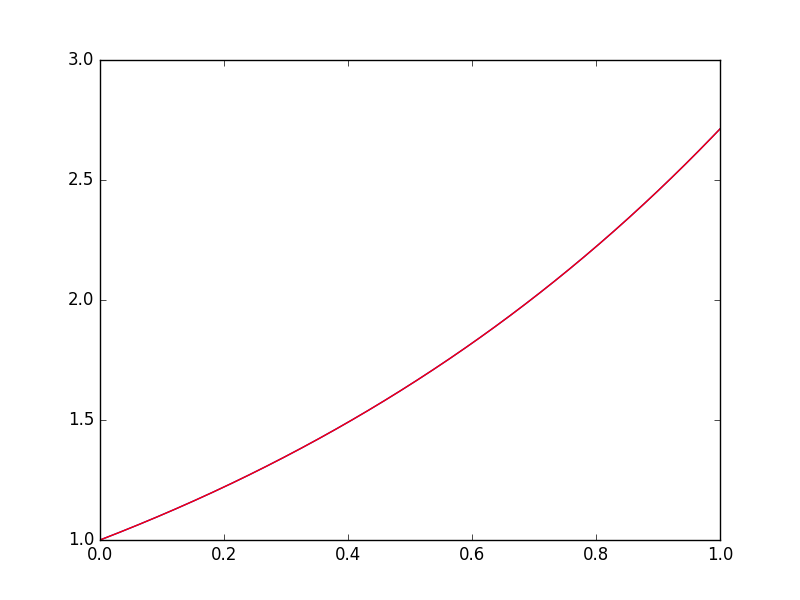
\includegraphics[scale=0.28]{5a.png}
  \caption{Wielomian interpolacyjny funkcji $e^x$ w przedziale $[0, 1]$ i stopniu $n = 5$.}
\endminipage\hfill
\minipage{0.32\textwidth}
  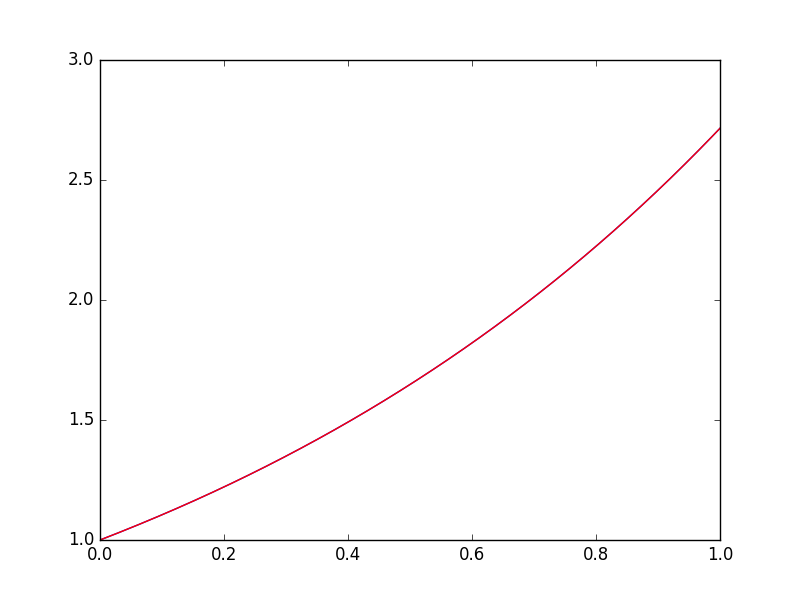
\includegraphics[scale=0.28]{5b.png}
  \caption{Wielomian interpolacyjny funkcji $e^x$ w przedziale $[0, 1]$ i stopniu $n = 10$.}
\endminipage\hfill
\minipage{0.32\textwidth}%
  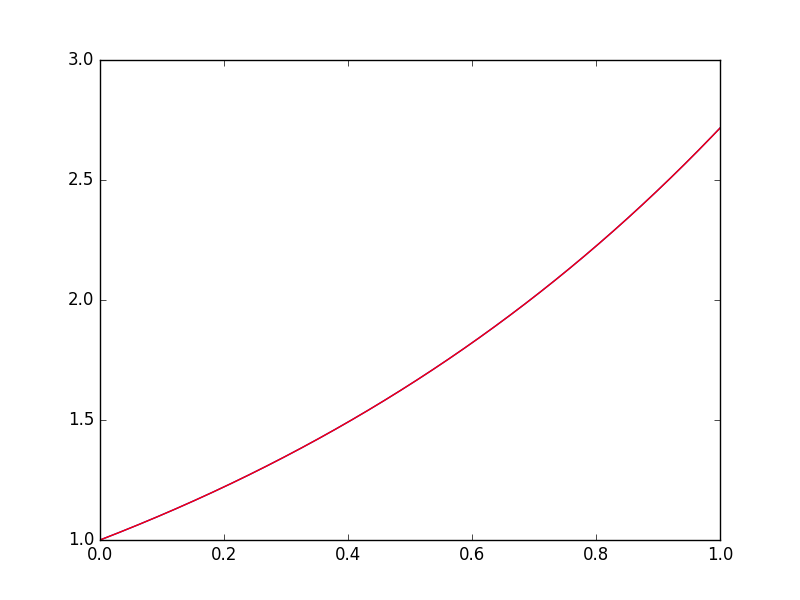
\includegraphics[scale=0.28]{5c.png}
  \caption{Wielomian interpolacyjny funkcji $e^x$ w przedziale $[0, 1]$ i stopniu $n = 15$.}
\endminipage
\end{figure}

Widoczne powyżej trzy wykresy niemal pokrywają się ze sobą. To niewielkie odchylenie jest widoczne dopiero po znacznym powiększeniu wykresu, na który zostały naniesione wszystkie trzy funkcje.

\begin{figure}[htbp]
  \centering
  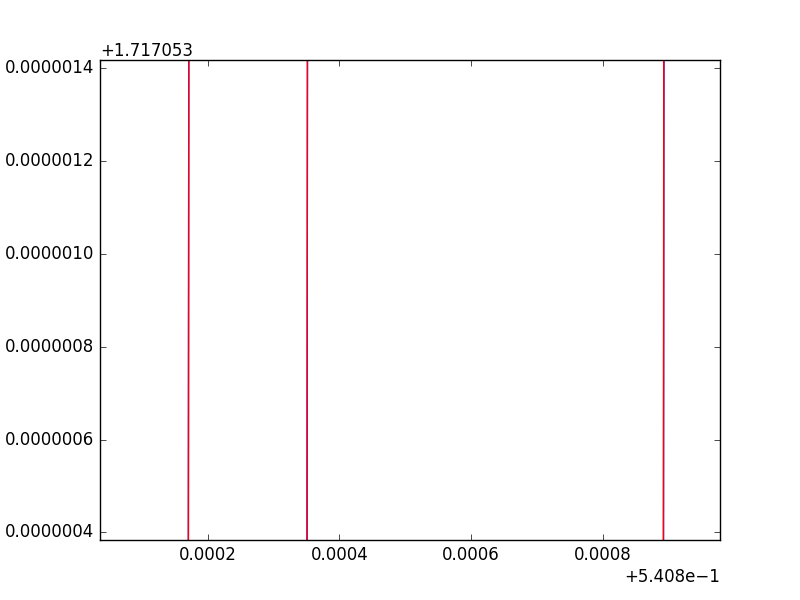
\includegraphics[scale=0.35]{5allA.png}
  \caption{Wielomiany interpolacyjne funkcji $e^x$ w przedziale $[0, 1]$ i stopniach $n = 5, 10, 15$.}
\end{figure}

Na powyższym wykresie widoczne są wykresy wielomianów interpolacyjnych dla zadanych stopni wielomianu. Jak widać odchylenie jest niewielkie, bo widoczne dopiero po znacznym powiększeniu wykresu.

\begin{figure}[!htb]
\minipage{0.32\textwidth}
  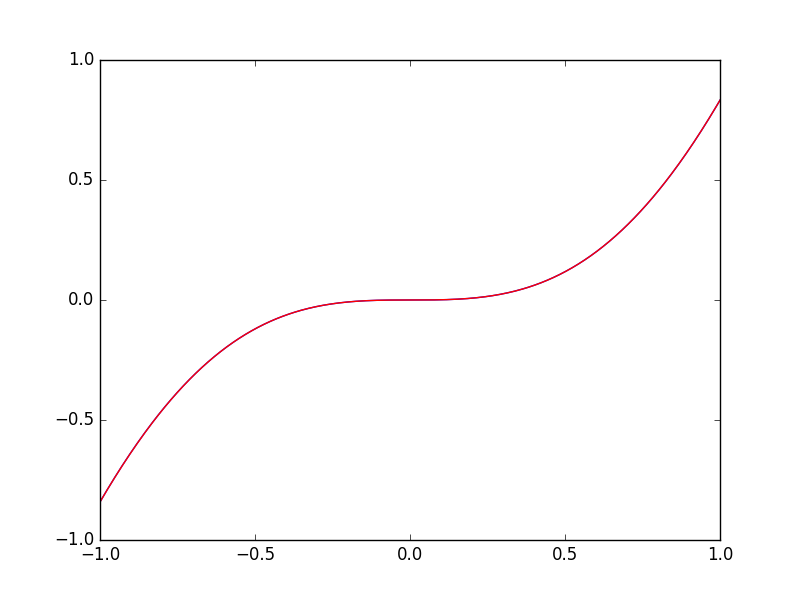
\includegraphics[scale=0.28]{5d.png}
  \caption{Wielomian interpolacyjny funkcji $x^2sinx(x)$ w przedziale $[-1, 1]$ i stopniu $n = 5$.}
\endminipage\hfill
\minipage{0.32\textwidth}
  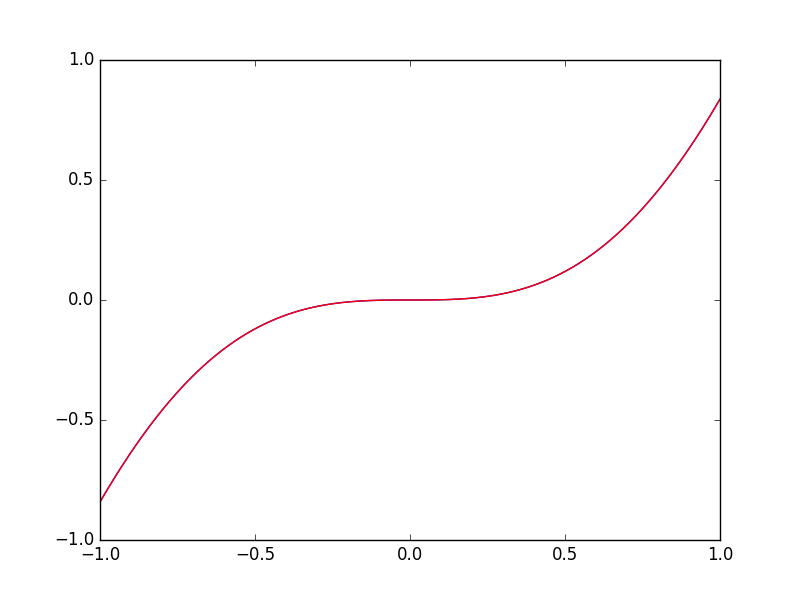
\includegraphics[scale=0.28]{5e.png}
  \caption{Wielomian interpolacyjny funkcji $x^2sinx(x)$ w przedziale $[-1, 1]$ i stopniu $n = 10$.}
\endminipage\hfill
\minipage{0.32\textwidth}%
  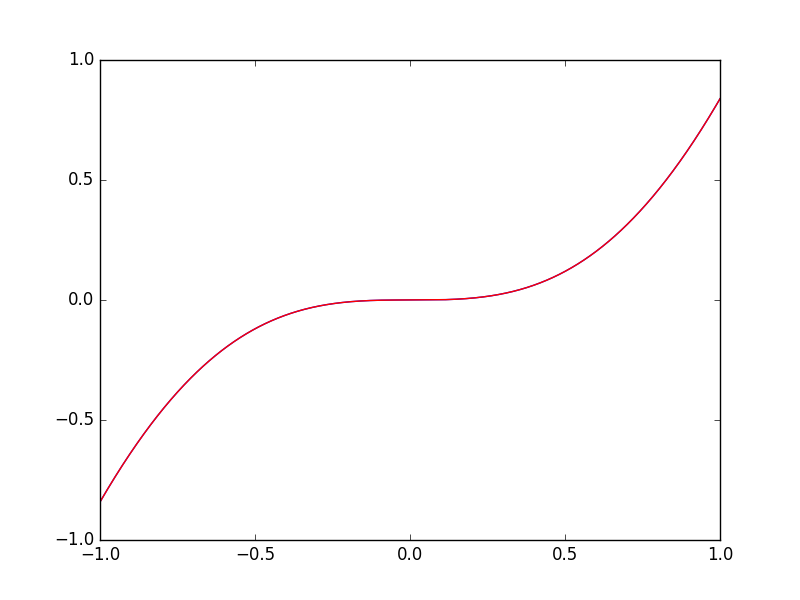
\includegraphics[scale=0.28]{5f.png}
  \caption{Wielomian interpolacyjny funkcji $x^2sinx(x)$ w przedziale $[-1, 1]$ i stopniu $n = 15$.}
\endminipage
\end{figure}

Również dla drugiej funkcji wielomiany interpolacyjne nie różnią się znacząco. Dopiero po powiększeniu wykresu, na który zostały naniesione trzy wielomiany interpolacyjne, są widoczne odchylenia.

\begin{figure}[htbp]
  \centering
  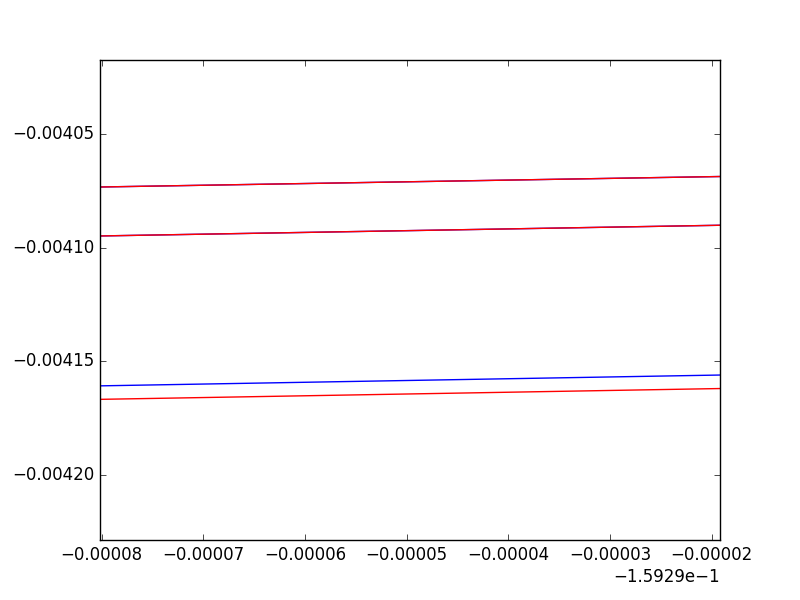
\includegraphics[scale=0.35]{5allB.png}
  \caption{Wielomiany interpolacyjne funkcji $x^2sinx(x)$ w przedziale $[-1, 1]$ i stopniach $n = 5, 10, 15$.}
\end{figure}

Na powyższym wykresie w kolorze czerwonym zostały narysowane wielomiany interpolacyjne funkcji $f(x) = x^2sinx(x)$, a kolorem niebieskim dokładne wartości tej funkcji. Jak widać odchylenia są niewielkie i widoczne dopiero po znacznym powiększeniu. Wielomianem, który jest najbardziej odchylony od wartości dokładnych jest wielomian o najniższym stopniu.
\subsection{Wnioski}
\paragraph{}
Dla wszystkich funkcji z zadanymi parametrami można było wyznaczyć wielomiany interpolacyjne, które niemal pokrywały się z dokładnymi wartościami funkcji. Małe odchylenia widoczne były dopiero po powiększeniu wykresów. Dla przykładów w zadaniu można również zauważyć, iż im większy stopień wielomianu interpolacyjnego, tym mniejsze odchylenie od wartości dokładnej.

\section{Zadanie szóste}

\subsection{Opis problemu}
\paragraph{}
Celem zadania było przetestowanie funkcji \texttt{rysujNnfx(f, a, b, n)} dla zadanych przykładów.

\subsection{Rozwiązanie}
\paragraph{}
Rozwiązanie zadania polegało na zaimportowaniu modułu stworzonego w ramach zadań od pierwszego do czwartego, a następnie wywołaniu funkcji \texttt{rysujNnfx(f, a, b, n)} z następującymi argumentami:

\begin{center}
\begin{itemize}
\item	Funkcja $|x|$ w przedziale $[-1, 1]$ i stopniem wielomianu interpolacyjnego $n = 5, 10, 15$.
\item	Funkcja $\frac{1}{1 + x^2}$ w przedziale $[-5, 5]$ i stopniem wielomianu interpolacyjnego $n = 5, 10, 15$.
\end{itemize}
\end{center}
\clearpage

\subsection{Wyniki i interpretacja}
\paragraph{}
\begin{figure}[!htb]
\minipage{0.32\textwidth}
  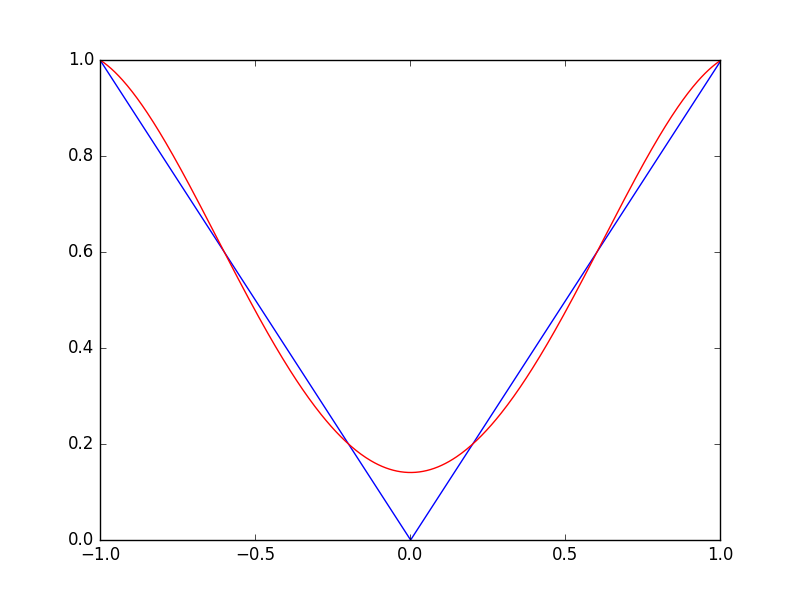
\includegraphics[scale=0.28]{6a.png}
  \caption{Wielomian interpolacyjny funkcji $|x|$ w przedziale $[-1, 1]$ i stopniu $n = 5$.}
\endminipage\hfill
\minipage{0.32\textwidth}
  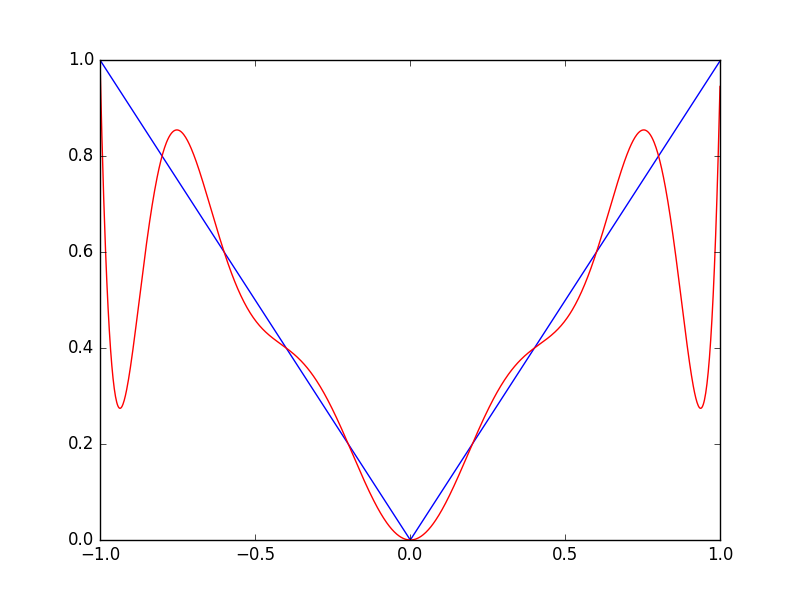
\includegraphics[scale=0.28]{6b.png}
  \caption{Wielomian interpolacyjny funkcji $|x|$ w przedziale $[-1, 1]$ i stopniu $n = 10$.}
\endminipage\hfill
\minipage{0.32\textwidth}%
  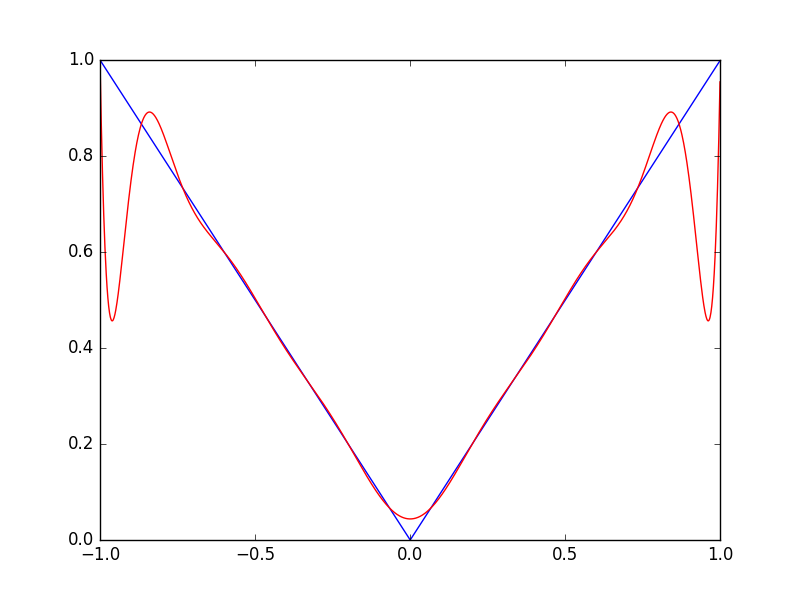
\includegraphics[scale=0.28]{6c.png}
  \caption{Wielomian interpolacyjny funkcji $|x|$ w przedziale $[-1, 1]$ i stopniu $n = 15$.}
\endminipage
\end{figure}

Na powyższych wykresach można zaobserwować, że wielomiany interpolacyjne nie są zbieżne do funkcji $f$. Odchylenie jest znacznie bardziej widoczne wraz ze zbliżaniem się wielomianu interpolacyjnego do krańców przedziału $[a, b]$.

\begin{figure}[htbp]
  \centering
  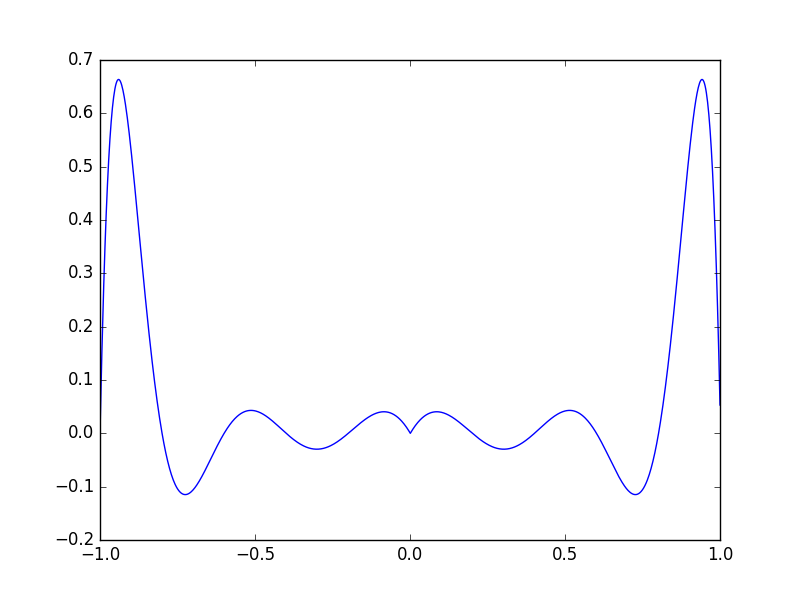
\includegraphics[scale=0.35]{6aError.png}
  \caption{Wykres błędu $e = f(x) - p(x)$, gdzie $f(x) = |x|$, a $p(x)$ to wielomian interpolacyjny stopnia $n = 10$.}
\end{figure}

Wykres błędu interpolacji wielomianowej potwierdza wcześniejsze obserwacje. Wraz ze zbliżaniem się do krańców przedziału interpolacji błąd rośnie. Błąd jest symetryczny względem $x = 0$, co wynika z charakterystyki funkcji $f(x) = |x|$. Przykład ten pokazuje również, że zwiększenie stopnia wielomianu interpolacyjnego nie musi powodować zmnieszenia błędu.
\clearpage

\begin{figure}[!htb]
\minipage{0.32\textwidth}
  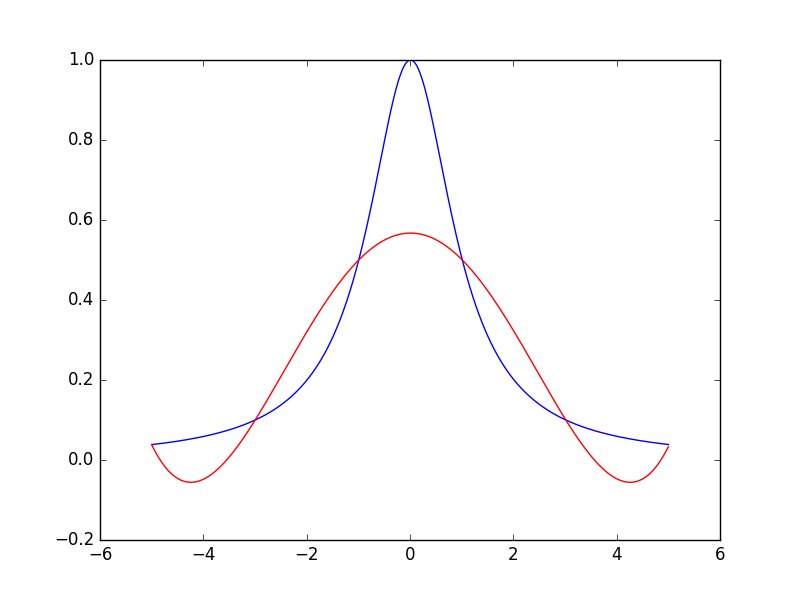
\includegraphics[scale=0.28]{6d.png}
  \caption{Wielomian interpolacyjny funkcji $\frac{1}{1 + x^2}$ w przedziale $[-1, 1]$ i stopniu $n = 5$.}
\endminipage\hfill
\minipage{0.32\textwidth}
  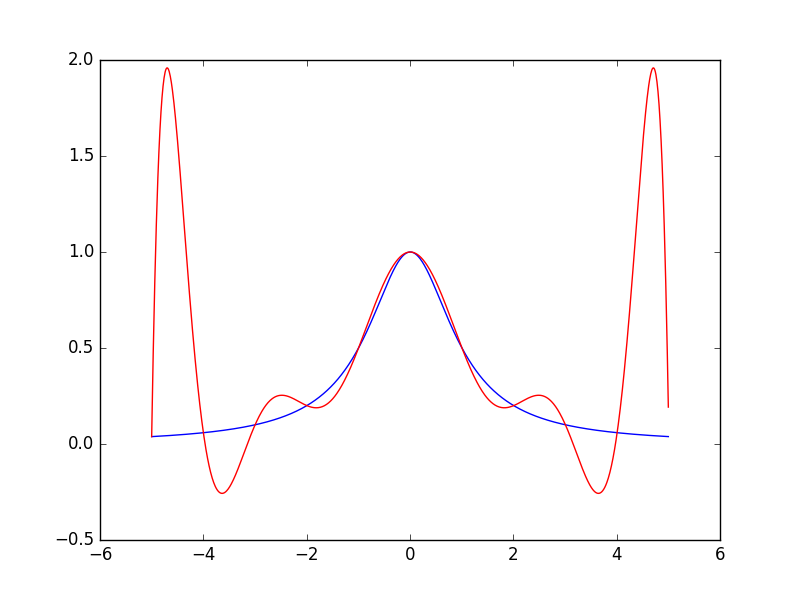
\includegraphics[scale=0.28]{6e.png}
  \caption{Wielomian interpolacyjny funkcji $\frac{1}{1 + x^2}$ w przedziale $[-1, 1]$ i stopniu $n = 10$.}
\endminipage\hfill
\minipage{0.32\textwidth}%
  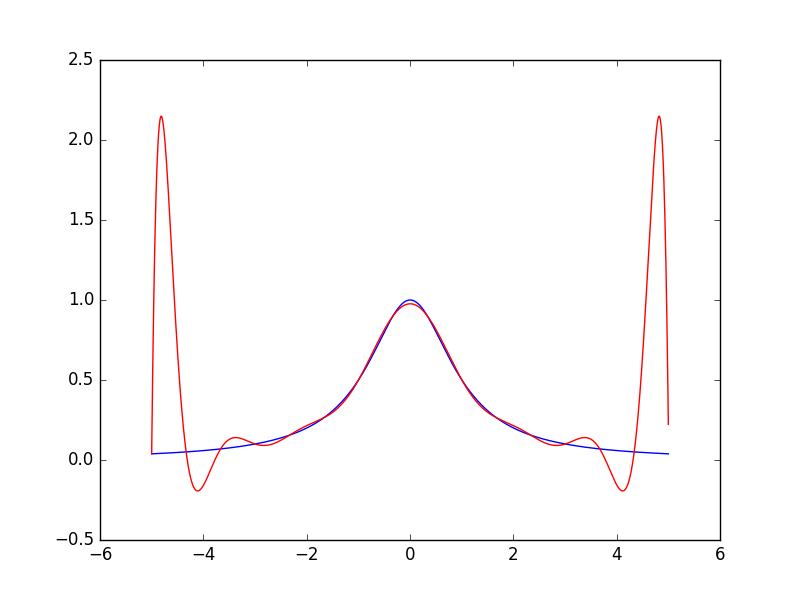
\includegraphics[scale=0.28]{6f.png}
  \caption{Wielomian interpolacyjny funkcji $\frac{1}{1 + x^2}$ w przedziale $[-1, 1]$ i stopniu $n = 15$.}
\endminipage
\end{figure}

Na powyższych wykresach można zaobserwować znaczne odchylenia od wartości dokładnej funkcji. Wraz ze zbliżaniem się do krańców przedziału wielomian interpolacyjny zaczyna gwałtowniej oscylować. Jest to zjawisko \textit{Rungego}. Początkowo wraz ze wzrostem liczby węzłów równoodległych dokładność zwiększa się, jednak dla większych $n$ przybliżenie pogarsza się, co jest widoczne szczególnie na krańcach przedziałów.

\begin{figure}[htbp]
  \centering
  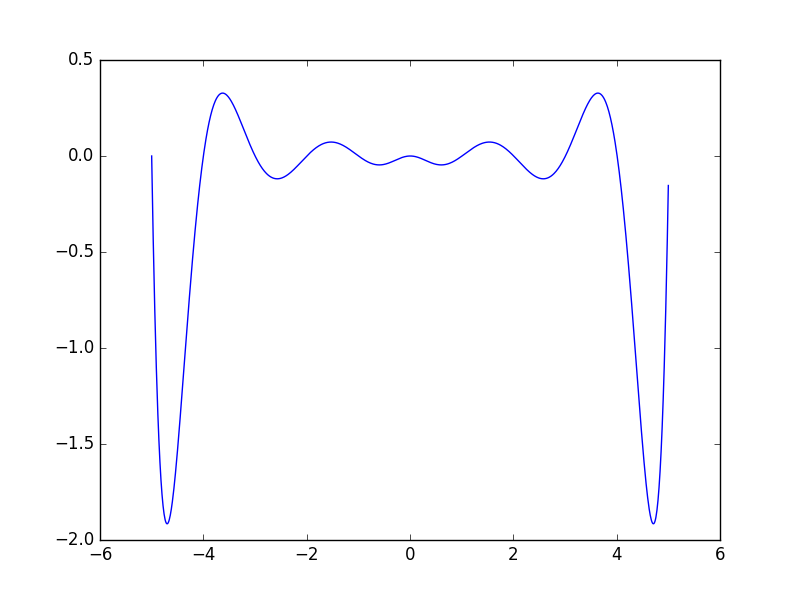
\includegraphics[scale=0.35]{6bError.png}
  \caption{Wykres błędu $e = f(x) - p(x)$, gdzie $f(x) = \frac{1}{1 + x^2}$, a $p(x)$ to wielomian interpolacyjny stopnia $n = 10$.}
\end{figure}

Tak silne oscylowanie na krańcach przedziału jest związane z dużymi błędami interpolacji. Przy interpolacji funkcji za pomocą wielomianów chcemy, aby błąd interpolacji dążył do zera wraz z $n \to \inf$. Dla powyższej funkcji $ max_{a \leq \xi_{x} \leq b} f^{n + 1}(\xi_{x})$ bardzo szybko dąży do nieskończoności wraz ze wzrostem $n$. Z tego powodu błąd interpolacji nie jest ograniczony od góry i zwiększa się wraz ze wzrostem $n$. Jest to spowodowane użyciem węzłów równoodległych. Wielomian oparty na węzłach równoodległych silnie oscyluje na krańcach przedziału, gdyż wielomian ten jest wysokiego stopnia, więc musi mieć dużo zer, a zarazem chce szybko uciec do nieskończoności. Oscylację możemy zredukować poprzez zastosowanie węzłów Czebyszewa, które są zagęszczone na krańcach przedziału i z tego powodu redukują występującą tam oscylację. 

\subsection{Wnioski}
\paragraph{}
W tym zadaniu, w przeciwieństwie do zadania piątego, zwiększenie stopnia wielomianu interpolacyjnego spowodowało generowanie większych odchyleń. Można było tutaj zaobserwować zjawiska rozbieżności wielomianów spowodowane doborem węzłów równoodległych lub samą charakterystyką funkcji.

\end{document}